\documentclass{beamer}

\usepackage[utf8]{inputenc}
\usepackage{lmodern} 
\usepackage[utf8]{inputenc}
\usepackage{lmodern} 
\usepackage{listings}
\usepackage{xcolor} 
\usepackage{graphicx}
\definecolor{myblue}{RGB}{48, 63, 159}
\setbeamercolor{palette primary}{bg=myblue, fg=white}
\setbeamercolor{structure}{fg=myblue}
\setbeamercolor{frametitle}{bg=myblue, fg=white}
\setbeamercolor{title}{bg=myblue, fg=white}
\setbeamercolor{footlinecolor}{bg=myblue, fg=white}


\defbeamertemplate*{title page}{mytemplate}{
	\vfill
	\begin{center}
		
		\begin{beamercolorbox}[wd=0.8\paperwidth, center, rounded=true, shadow=true]{title}
			\usebeamerfont{title}\inserttitle\par
		\end{beamercolorbox}
		\vspace{2cm} 
		
		\usebeamerfont{author}\insertauthor
		\vspace{1cm} 
		\usebeamerfont{date}\insertdate
	\end{center}
	\vfill
}


\defbeamertemplate*{frametitle}{mytemplate}{
	\begin{beamercolorbox}[wd=\paperwidth, ht=2.5ex, dp=1.5ex, left]{frametitle}
		\hspace{1em}\usebeamerfont{frametitle}\insertframetitle
	\end{beamercolorbox}
}


\setbeamertemplate{footline}{
	\begin{beamercolorbox}[wd=\paperwidth, ht=2.25ex, dp=1ex]{footlinecolor}
		\hspace{1em}\usebeamerfont{author in footline}\insertshortauthor
		\hfill
		\usebeamerfont{title in footline}\insertshorttitle
		\hfill
		\usebeamerfont{date in footline}\insertdate \hspace{1em} \insertframenumber/\inserttotalframenumber \hspace{0.5em}
	\end{beamercolorbox}
}


\setbeamerfont{author in footline}{size=\tiny}
\setbeamerfont{title in footline}{size=\tiny}
\setbeamerfont{date in footline}{size=\tiny}

\newcommand{\myvec}[1]{\ensuremath{\begin{pmatrix}#1\end{pmatrix}}}
\providecommand{\brak}[1]{\ensuremath{\left(#1\right)}}


\title{9.6.2}
\author{Shriyansh Chawda-EE25BTECH11052}




\begin{document}
	

		\setbeamertemplate{footline}{} 
		\frame{\titlepage}
	
	
	

	\begin{frame}{Question} 
Find the area of the circle $4x^{2} + 4y^{2} = 9$ which is interior to the parabola $x^{2} = 4y.$\\
\end{frame}
	
\begin{frame}{Solution}
The conic parameters for the two curves can be expressed as follows:\\
For the circle $4x^2 + 4y^2 - 9 = 0$:
\begin{align}
	\mathbf{V_1} = \myvec{4 & 0 \\ 0 & 4}, \mathbf{u_1} = \myvec{0 \\ 0}, f_1 = -9. 
\end{align}
For the parabola $x^2 - 4y = 0$:
\begin{align}
	\mathbf{V_2} = \myvec{1 & 0 \\ 0 & 0}, \mathbf{u_2} = \myvec{0 \\ -2}, f_2 = 0. 
\end{align}
The intersection of two conics with parameters $\mathbf{V_i}$, $\mathbf{u_i}$, $f_i$, i = 1, 2 is defined as:
\end{frame}



\begin{frame}{Solution}
\begin{equation}
	\mathbf{x}^\top(\mathbf{V_1} + \mu\mathbf{V_2})\mathbf{x} + 2(\mathbf{u_1} + \mu\mathbf{u_2})^\top\mathbf{x} + (f_1 + \mu f_2) = 0 
\end{equation}
For a degenerate conic, the determinant of the quadratic part's matrix must be zero.
\begin{align}
	&\det(\mathbf{V_1} + \mu\mathbf{V_2}) = 0 \\
	&\det\left(\myvec{4 & 0 \\ 0 & 4} + \mu\myvec{1 & 0 \\ 0 & 0}\right) =
	\begin{vmatrix}
		4+\mu & 0 \\
		0 & 4
	\end{vmatrix}
	= 4(4+\mu) = 0 \\
	&\mu = -4
\end{align}
Substituting $\mu = -4$ in (3) :
\end{frame}

\begin{frame}{Solution}
 \begin{align} 
 	&\mathbf{x}^\top( \mathbf{V_1} - 4\mathbf{V_2} )\mathbf{x} + 2( \mathbf{u_1} - 4\mathbf{u_2} )^\top\mathbf{x} + ( f_1 - 4f_2 ) = 0 \\
 	&\mathbf{x}^\top\left( \myvec{4 & 0 \\ 0 & 4} - 4\myvec{1 & 0 \\ 0 & 0} \right)\mathbf{x} + 2\left( \myvec{0 \\ 0} - 4\myvec{0 \\ -2} \right)^\top\mathbf{x} + ( -9 - 4(0) ) = 0 \\
 	&\mathbf{x}^\top \myvec{0 & 0 \\ 0 & 4} \mathbf{x} + 2 \myvec{0 \\ 8}^\top \mathbf{x} - 9 = 0 
 \end{align}
 Letting $\mathbf{x} = \myvec{x \\ y}$, the equation becomes:
 \begin{align} \myvec{x & y} \myvec{0 & 0 \\ 0 & 4} \myvec{x \\ y} + 2 \myvec{0 & 8} \myvec{x \\ y} - 9 = 0 \end{align}
 \begin{align} \implies 4y^2 + 16y - 9 = 0 \end{align}
\end{frame}

\begin{frame}{Solution}
Solving for y yields $y = 1/2$ and $y = -9/2$. For the area to be interior to the parabola $x^2 = 4y$, we must have $y \ge 0$. Therefore, the intersection occurs at the line $y = 1/2$. Substituting $y = 1/2$ into the parabola's equation:
\begin{align} x^2 = 4(1/2) = 2 \implies x = \pm\sqrt{2}. \end{align}
Hence, the points of intersection are:
\begin{align} 
	\mathbf{a_1} = \myvec{\sqrt{2} \\ 1/2}, \mathbf{a_2} = \myvec{-\sqrt{2} \\ 1/2}
\end{align}
The desired area of the region is given by:
\begin{align} A = \int_{-\sqrt{2}}^{\sqrt{2}} \left( \sqrt{\frac{9}{4} - x^2} - \frac{x^2}{4} \right) dx \
\end{align}
\end{frame}



\begin{frame}{Solution}
Due to symmetry,
\begin{align}
	&= 2 \left[ \int_{0}^{\sqrt{2}} \sqrt{\frac{9}{4} - x^2} \, dx - \int_{0}^{\sqrt{2}} \frac{x^2}{4} \, dx \right] \\
	\intertext{The first integral uses the standard formula for $\sqrt{a^2-x^2}$ (from trig substitution).}
	\int_{0}^{\sqrt{2}} \sqrt{\frac{9}{4} - x^2} \, dx &= \frac{\sqrt{2}}{4} + \frac{9}{8}\sin^{-1}\left(\frac{2\sqrt{2}}{3}\right) 
	\intertext{The second integral uses the simple power rule.}
	\int_{0}^{\sqrt{2}} \frac{x^2}{4} \, dx &= \frac{\sqrt{2}}{6} 
\end{align}
\end{frame}

\begin{frame}{Solution}
\begin{align}
\intertext{Substituting these results back:}
A &= 2 \left[ \left( \frac{\sqrt{2}}{4} + \frac{9}{8}\sin^{-1}\left(\frac{2\sqrt{2}}{3}\right) \right) - \frac{\sqrt{2}}{6} \right] \\
A &= \frac{\sqrt{2}}{6} + \frac{9}{4}\sin^{-1}\left(\frac{2\sqrt{2}}{3}\right)
\end{align}
\end{frame}

\begin{frame}{Plot}
\begin{figure}[H]
	\centering
	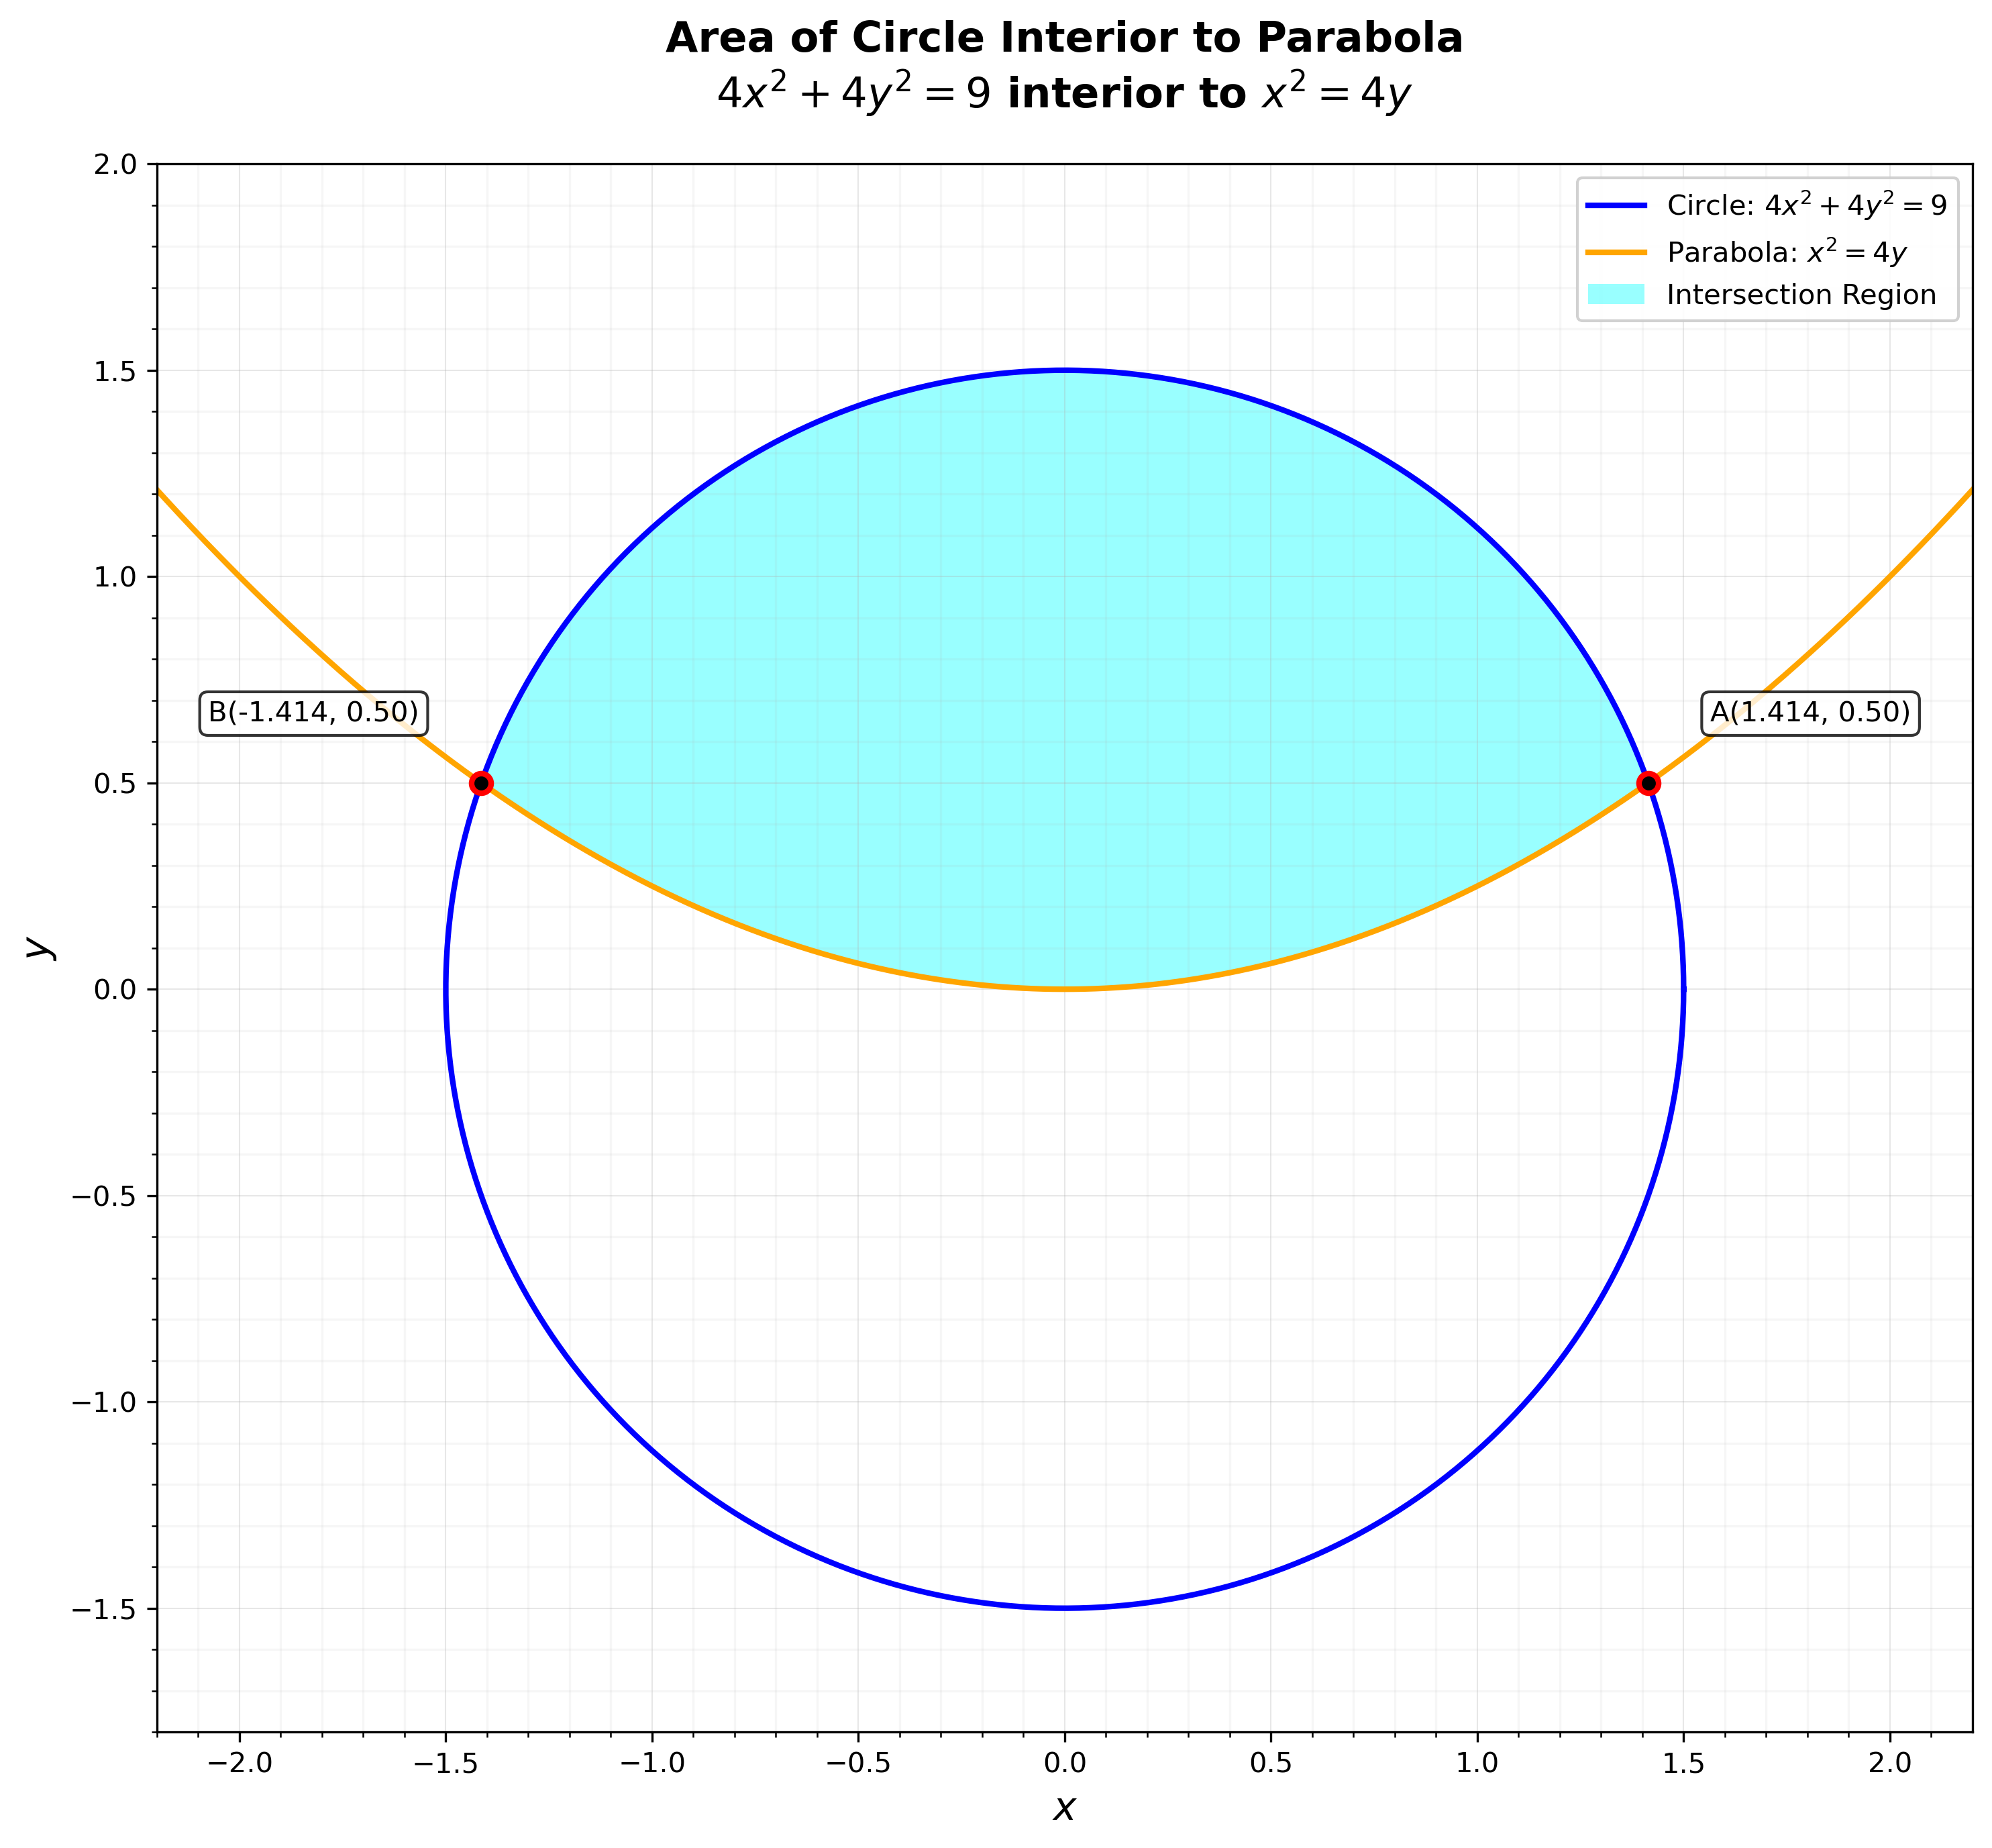
\includegraphics[width=0.83\linewidth]{figs/area_plot}
	\caption{}
	\label{fig:areaplot}
\end{figure}

\end{frame}
\end{document}